\section{Experiment}\label{sec:exp}

In this section, we detail the training and inference setup of AURA, report its benchmark accuracy and inference performance, and present additional experimental analyses.

\subsection{Implementation Details}
\label{subsec:training_detail}

\begin{figure}[t]
    \centering
    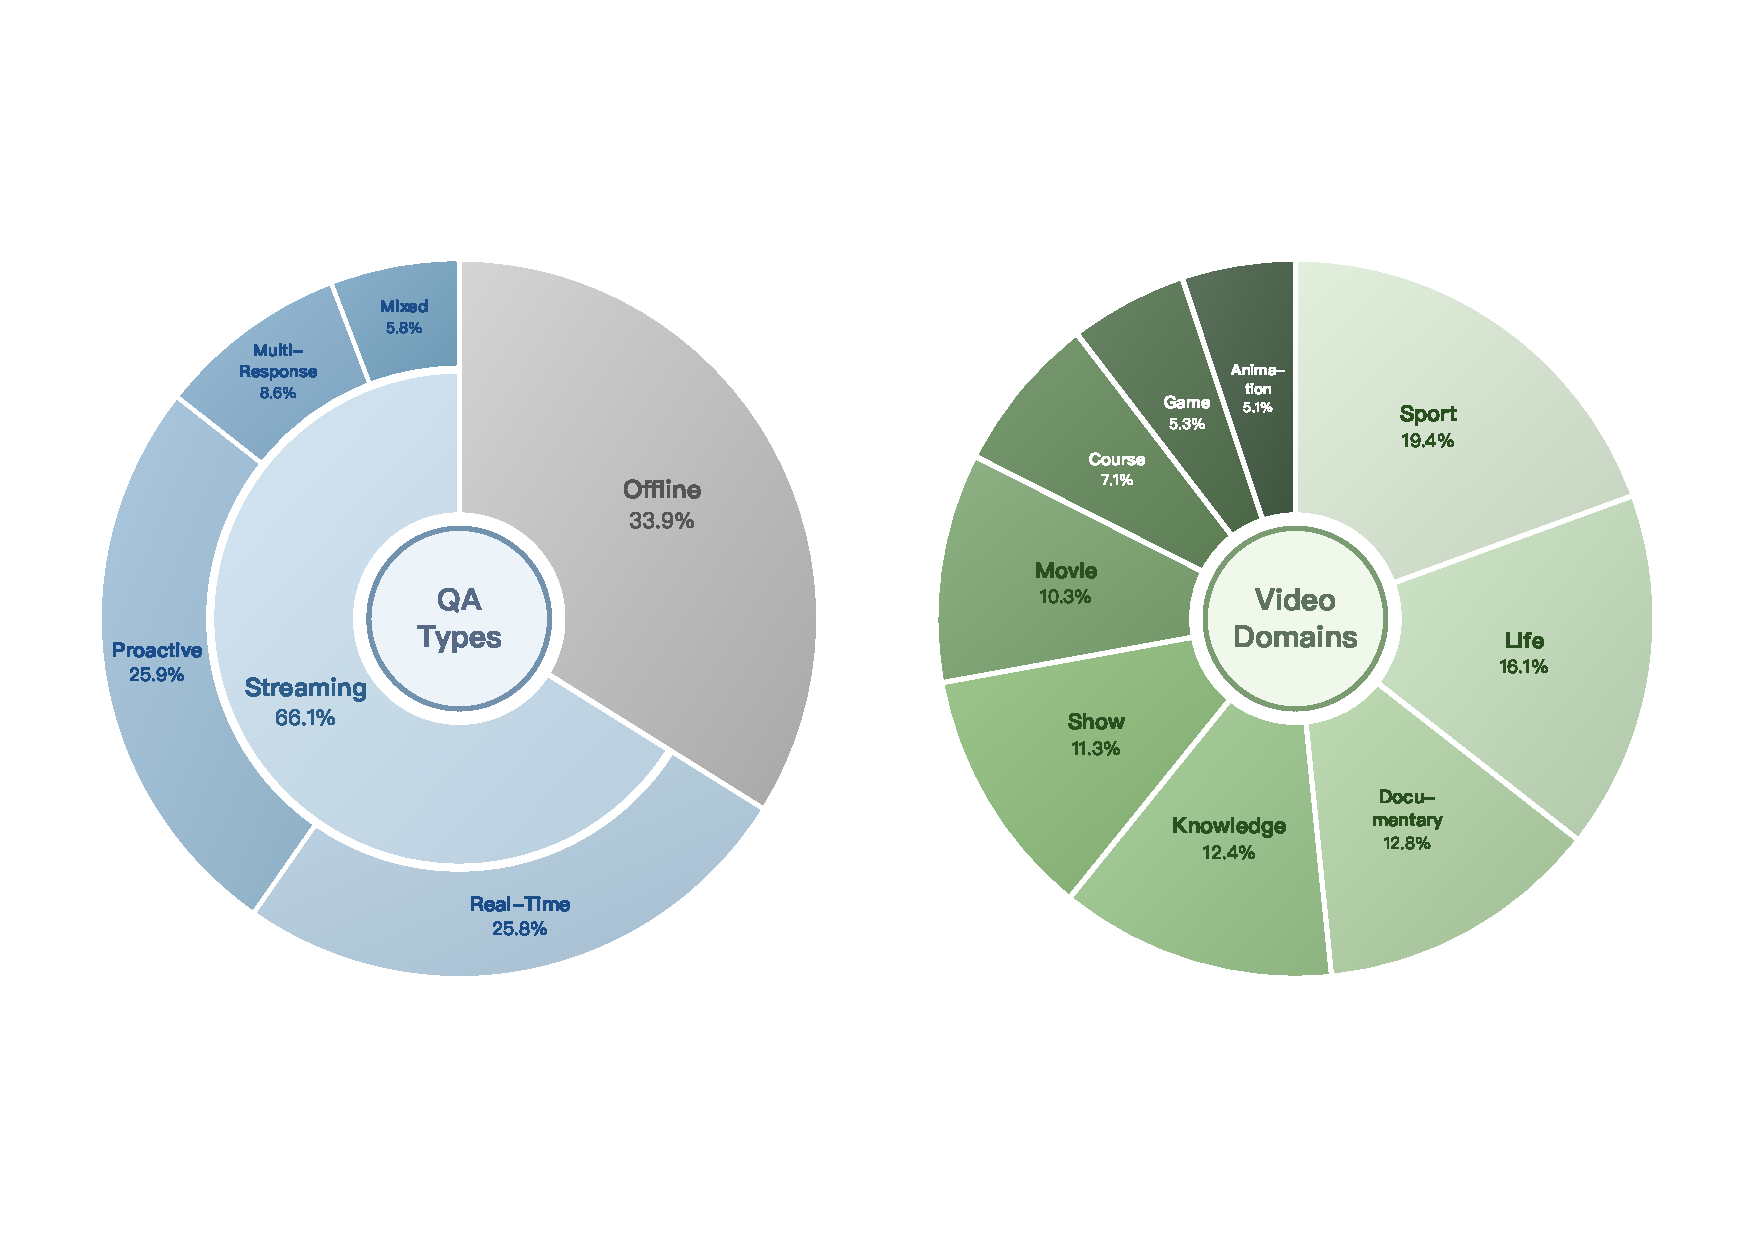
\includegraphics[width=0.9\textwidth]{img/6_data_distribution_2.pdf}
    \caption{Training data distribution: Left: QA type distribution; Right: Video domain distribution. It shows that the training set covers diverse question formats and video domains.}
    \label{fig:data_distribution}
\end{figure}

\begin{table*}[t]
  \renewcommand{\arraystretch}{1.3}
  \caption{Quantitative comparison on StreamingBench in terms of accuracy (\%). We report performance on each fine-grained task, along with the average results for Real-Time Visual Understanding (RTVU), Omni-Source Understanding (OSU), Contextual Understanding (CU), and the overall average. The best and second-best results are highlighted in bold and underlined, respectively.}
  \label{tab:streamingbench}
  \centering
  \resizebox{\textwidth}{!}{%
  \setlength{\tabcolsep}{2pt}%
  \footnotesize
  \begin{tabular}{l|l*{21}{c}}
    \toprule
    \multirow{2}{*}{Method} & \multicolumn{11}{c}{\textbf{RTVU}} & \multicolumn{5}{c}{\textbf{OSU}} & \multicolumn{5}{c}{\textbf{CU}} & \multirow{2}{*}{\textbf{All}} \\
    \cmidrule(lr){2-12}
    \cmidrule(lr){13-17}
    \cmidrule(lr){18-22}
    & OP & CR & CS & ATP & EU & TR & PR & SU & ACP & CT & Avg & ER & SCU & SD & MA & Avg & MCU & ACU & SQA & PO & Avg & \\
    \midrule
    \multicolumn{23}{c}{\textit{Proprietary Models}} \\
    \midrule
    GPT-4o & 77.1 & 80.5 & 83.9 & 76.5 & 70.2 & 83.8 & 66.7 & 62.2 & 69.1 & 49.2 & 73.3 & 41.2 & 37.2 & 43.6 & 56.0 & 44.5 & 41.2 & 38.4 & 32.8 & 56.9 & 38.7 & 60.2 \\
    Gemini-1.5-Pro & 79.0 & 80.5 & 83.5 & 79.7 & 80.0 & 84.7 & 77.8 & 64.2 & 72.0 & 48.7 & 75.7 & 46.8 & 39.6 & 74.9 & 80.0 & 60.2 & 51.4 & 40.7 & 54.8 & 45.1 & 48.7 & 67.1 \\
    \midrule
    \multicolumn{23}{c}{\textit{Open-Source Models}} \\
    \midrule
    StreamAgent & 79.6 & 78.3 & 79.3 & 75.9 & 74.7 & 76.9 & \underline{82.9} & 66.3 & 73.7 & 55.4 & 74.3 & 35.9 & 26.3 & 38.9 & 44.0 & 36.3 & 39.7 & 30.3 & 39.6 & 28.9 & 34.6 & 57.0 \\
    ViSpeak & 79.8 & 71.1 & 81.4 & 78.8 & 74.5 & 70.1 & 63.9 & 64.2 & 71.4 & 28.0 & 70.4 & \underline{47.2} & \textbf{56.4} & \underline{61.6} & \textbf{81.2} & \underline{61.6} & \underline{49.2} & 36.4 & 39.2 & 50.8 & 43.9 & 62.6 \\
    Qwen3-VL-8B-Inst. & 80.1 & 76.6 & 81.1 & 81.1 & 77.0 & 73.2 & 80.6 & 63.4 & 68.8 & \textbf{57.0} & 74.1 & 44.4 & 27.2 & 46.4 & 49.6 & 41.9 & 30.0 & 38.4 & 38.0 & \underline{52.8} & 39.8 & 59.3 \\
    MiniCPM-o-4.5 & \underline{80.9} & \textbf{88.3} & \underline{82.0} & \underline{85.0} & \underline{78.9} & \underline{85.4} & 78.7 & \underline{67.1} & \underline{75.6} & \underline{56.0} & \underline{78.2} & 44.4 & 28.0 & 41.6 & 54.4 & 42.1 & 35.2 & \underline{44.0} & \underline{51.2} & 47.6 & \underline{44.5} & \underline{62.7} \\
    AURA (Ours) & \textbf{87.5} & \underline{84.4} & \textbf{93.4} & \textbf{89.5} & \textbf{83.2} & \textbf{87.9} & \textbf{86.1} & \textbf{76.4} & \textbf{82.4} & 47.7 & \textbf{83.2} & \textbf{56.4} & \underline{48.4} & \textbf{62.8} & \underline{80.4} & \textbf{62.0} & \textbf{54.8} & \textbf{70.8} & \textbf{57.2} & \textbf{53.2} & \textbf{59.0} & \textbf{73.1} \\
    
    \bottomrule
  \end{tabular}%
  }
\end{table*}


All experiments are conducted on a computing cluster equipped with high-performance accelerators with 80 GB of HBM3 memory. Training is performed on 4 nodes with 8 accelerators per node (32 accelerators in total). We initialize our model from Qwen3-VL-8B-Instruct~\citep{bai2025qwen3} and fine-tune only the LLM component while keeping the vision encoder and the connector frozen. The training data include approximately 115k streaming video QA samples (about 1.04B tokens), constructed using the data pipeline described in Section~\ref{sec:data_pipe}, as well as approximately 59k in-house offline video QA samples (about 0.16B tokens). In total, the training set contains approximately 174k samples, corresponding to about 1.2B tokens. Detailed data distributions are shown in Figure~\ref{fig:data_distribution}. The model is trained for one epoch with a global batch size of 128 and a learning rate of $1\times10^{-5}$. For context management, the video chunk size is set to 1 second, and the hyperparameters $N$, $N'$, and $M$ are set to 30, 15, and 10, respectively.

\subsection{Evaluation Protocol}

\paragraph{Benchmarks.}
We evaluate our AURA on three streaming video understanding benchmarks: StreamingBench~\citep{lin2024streamingbench}, OVO-Bench~\citep{niu2025ovo}, and OmniMMI~\citep{wang2025omnimmi}. StreamingBench is a comprehensive benchmark designed to evaluate streaming video understanding capabilities of VideoLLMs, focusing on real-time visual understanding, omni-source understanding, and contextual understanding through multi-timestamp question answering on continuous video streams. OVO-Bench emphasizes temporal awareness in online video understanding and evaluates models under backward tracing, real-time understanding, and forward active responding scenarios using fine-grained timestamp annotations. OmniMMI is a comprehensive multimodal interaction benchmark for streaming video contexts, which evaluates not only streaming video understanding but also proactive reasoning and multimodal interaction abilities across multiple tasks.

\paragraph{Evaluation Pipeline.}\label{Eval_pipe}

We conduct all evaluations on computing nodes with the same specifications as those used for training, and use the official codebases for the corresponding benchmarks~\citep{lin2024streamingbench,niu2025ovo,wang2025omnimmi}. We manage model context using our Interactive Video Stream Context Management mechanism. For other models, we report official results when complete results are publicly available~\citep{fu2025vispeak, wang2025omnimmi, xia2025streaming, yang2025streamagent}; otherwise, we evaluate them by strictly following the code released in the official benchmark repositories~\citep{minicpmo45,bai2025qwen3}. We also note that, although MiniCPM-o-4.5 supports a full-duplex multimodal live-streaming mode, we find that it often becomes silent in this setting and may produce irrelevant responses for video streams longer than two minutes. Therefore, we do not use this mode in our evaluation.

\subsection{Main Result}


We compare AURA with strong proprietary baselines, including GPT-4o~\citep{hurst2024gpt} and Gemini-1.5-Pro~\citep{team2024gemini}, as well as open-source baselines, including StreamAgent~\citep{yang2025streamagent}, Streamo-7B~\citep{xia2025streaming}, ViSpeak~\citep{fu2025vispeak}, M4~\citep{wang2025omnimmi}, Qwen3-VL-8B-Instruct~\citep{bai2025qwen3}, and MiniCPM-o-4.5~\citep{minicpmo45}, on three representative streaming video benchmarks. As shown in Tables~\ref{tab:streamingbench},~\ref{tab:ovobench}, and~\ref{tab:omnimmi}, AURA achieves the best overall performance on all three benchmarks, demonstrating strong capability in streaming scenarios.

\begin{table*}[t]
  \renewcommand{\arraystretch}{1.3}
  \caption{Quantitative comparison on OVO-Bench in terms of accuracy (\%). We report performance on each fine-grained task, along with the average results for Real-Time Visual Perception (RTVP), Backward Tracing (BT), Forward Active Responding (FAR), and the overall average. The best and second-best results are highlighted in bold and underlined, respectively.}
  \label{tab:ovobench}
  \centering
  \setlength{\tabcolsep}{3.5pt}%
  \footnotesize
  \begin{tabular}{l|l*{15}{c}}
    \toprule
    \multirow{2}{*}{Method} & \multicolumn{7}{c}{\textbf{RTVP}} & \multicolumn{4}{c}{\textbf{BT}} & \multicolumn{4}{c}{\textbf{FAR}} & \multirow{2}{*}{\textbf{All}} \\
    \cmidrule(lr){2-8}
    \cmidrule(lr){9-12}
    \cmidrule(lr){13-16}
    & OCR & ACR & ATR & STU & FPD & OJR & Avg & EPM & ASI & HLD & Avg & REC & SSR & CRR & Avg & \\
    \midrule
    \multicolumn{17}{c}{\textit{Proprietary Models}} \\
    \midrule
    GPT-4o & 69.8 & 64.2 & 71.6 & 51.1 & 70.3 & 59.8 & 64.5 & 57.9 & 75.7 & 48.7 & 60.8 & 73.2 & 27.6 & 59.4 & 53.4 & 59.5 \\
    Gemini-1.5-Pro & 85.9 & 67.0 & 79.3 & 58.4 & 63.4 & 62.0 & 69.3 & 58.6 & 76.4 & 52.6 & 62.5 & 35.5 & 74.2 & 61.7 & 57.2 & 63.0 \\
    \midrule
    \multicolumn{17}{c}{\textit{Open-Source Models}} \\
    \midrule
    StreamAgent & 71.2 & 53.2 & 63.6 & 53.9 & 67.3 & 58.7 & 61.3 & 54.8 & 58.1 & 25.8 & 41.7 & \underline{35.9} & 48.4 & 52.0 & 45.4 & 49.4 \\
    Streamo-7B & \underline{77.2} & \underline{66.1} & \underline{76.7} & 45.5 & 66.3 & \underline{72.8} & \underline{67.4} & 55.6 & 58.1 & 33.9 & 49.2 & 30.8 & 57.6 & \textbf{82.5} & \textbf{57.0} & 57.9 \\
    ViSpeak & 75.2 & 58.7 & 71.6 & 51.1 & \underline{74.3} & 66.9 & 66.3 & \textbf{59.9} & 48.7 & \textbf{64.0} & \underline{57.5} & 33.8 & \underline{68.5} & 60.4 & 54.3 & \underline{61.1} \\
    MiniCPM-o-4.5 & 73.2 & 65.1 & 75.0 & 59.0 & 69.3 & 62.5 & 67.3 & 55.2 & \underline{66.9} & 45.7 & 55.9 & \textbf{43.0} & 66.0 & 58.8 & \underline{55.9} & 59.7 \\
    Qwen3-VL-8B-Inst. & 54.5 & 58.7 & 68.5 & \textbf{70.3} & 68.1 & 49.5 & 61.6 & \underline{58.8} & 41.1 & 23.1 & 41.0 & 21.2 & 51.3 & 40.4 & 37.7 & 46.8 \\
    AURA (Ours) & \textbf{89.9} & \textbf{79.8} & \textbf{80.2} & \underline{70.2} & \textbf{77.2} & \textbf{81.5} & \textbf{79.8} & 54.9 & \textbf{67.6} & \underline{58.6} & \textbf{60.4} & 30.4 & \textbf{75.8} & \underline{61.3} & 55.8 & \textbf{65.3} \\
    \bottomrule
  \end{tabular}%
\end{table*}

\begin{table*}[t]
  \renewcommand{\arraystretch}{1.3}
  \caption{Quantitative comparison on OmniMMI in terms of accuracy (\%). We report performance for Dynamic State Grounding (SG), Action Prediction (AP), Multi-turn Dependency Reasoning (MD), Speaker Identification (SI), Proactive Alerting (PA), and the overall average. The best and second-best results are highlighted in bold and underlined, respectively.}
  \label{tab:omnimmi}
  \centering
  \setlength{\tabcolsep}{4pt}%
  \footnotesize
  \begin{tabular}{l|l*{11}{c}}
    \toprule
    \multirow{2}{*}{Method} & \multicolumn{4}{c}{\textbf{SG}} & \multirow{2}{*}{\textbf{AP}} & \multicolumn{4}{c}{\textbf{MD}} & \multirow{2}{*}{\textbf{SI}} & \multirow{2}{*}{\textbf{PA}} & \multirow{2}{*}{\textbf{All}} \\
    \cmidrule(lr){2-5}
    \cmidrule(lr){7-10}
    & 1st & 2nd & 3rd & Avg & & 1st & 2nd & 3rd & Avg & & & \\
    \midrule
    \multicolumn{13}{c}{\textit{Proprietary Models}} \\
    \midrule
    GPT-4o & 48.7 & 17.0 & 5.6 & 15.0 & 39.5 & 34.3 & 15.6 & 7.7 & 12.3 & 17.0 & \ding{55} & 16.8 \\
    Gemini-1.5-Pro & 52.3 & 19.7 & 9.4 & 16.3 & 43.0 & 35.0 & 16.3 & 7.1 & 12.0 & 38.5 & \ding{55} & 22.0 \\
    \midrule
    \multicolumn{13}{c}{\textit{Open-Source Models}} \\
    \midrule
    M4 & 35.7 & 6.4 & \underline{1.9} & 5.7 & \underline{33.5} & 35.7 & 6.4 & 1.9 & 1.7 & 9.0 & \underline{25.5} & 15.1 \\
    MiniCPM-o-4.5 & 46.3 & 8.1 & 0.9 & 6.3 & 25.0 & \underline{36.0} & \textbf{13.5} & \textbf{5.1} & \underline{9.3} & 17.0 & \ding{55} & 11.5 \\
    Qwen3-VL-8B-Inst. & \underline{51.3} & \underline{9.5} & 0.0 & \underline{7.7} & \textbf{36.5} & 33.7 & 11.1 & 3.5 & \textbf{9.7} & \textbf{29.5} & \ding{55} & \underline{16.7} \\
    AURA (Ours) & \textbf{52.7} & \textbf{26.4} & \textbf{15.0} & \textbf{24.0} & 32.0 & \textbf{37.3} & \underline{12.8} & \underline{3.6} & 7.7 & \underline{26.0} & \textbf{37.5} & \textbf{25.4} \\
    \bottomrule
  \end{tabular}%
\end{table*}

\paragraph{Performance Comparison.}

As reported in Table~\ref{tab:streamingbench}, AURA achieves the highest overall accuracy of 73.1\% on StreamingBench~\citep{lin2024streamingbench}, outperforming the strongest open-source baseline, MiniCPM-o-4.5, by 10.4\%. More importantly, this advantage is broad rather than concentrated on a few tasks. AURA ranks first among open-source models across all three high-level groups, \ie, Real-Time Visual Understanding (RTVU), Omni-Source Understanding (OSU), and Contextual Understanding (CU), and on 14 of the 18 fine-grained sub-tasks. AURA is also highly competitive with proprietary models, surpassing Gemini-1.5-Pro by 6.0\% overall (73.1\% vs.\ 67.1\%), while leading all proprietary models on the three group averages and on 15 of the 18 fine-grained sub-tasks.

This strong advantage generalizes to OVO-Bench~\citep{niu2025ovo}, as reported in Table~\ref{tab:ovobench}. AURA again obtains the highest overall accuracy of 65.3\%, improving over the best open-source result from ViSpeak by 4.2\%. At a finer granularity, AURA is the best open-source model on 2 of the 3 high-level settings, namely Real-Time Visual Perception (RTVP) and Backward Tracing (BT), and it trails the best model by only 1.2\% on Forward Active Responding (FAR). Compared with proprietary models, AURA remains competitive and even achieves a higher overall score than Gemini-1.5-Pro by 2.3\% (65.3\% vs.\ 63.0\%).

The same trend is also observed on OmniMMI~\citep{wang2025omnimmi}, as shown in Table~\ref{tab:omnimmi}, where AURA achieves the best overall accuracy of 25.4\%, surpassing all open-source and proprietary models. It ranks first on 5 of the 9 fine-grained metrics. It should be noted that non-streaming models (including MiniCPM-o-4.5 in non-duplex mode) do not have Proactive Alerting (PA) capability, and therefore PA is left blank.


\subsection{Inference Performance}





\paragraph{Inference Performance of AURA.}

\begin{figure}[t]
    \centering
    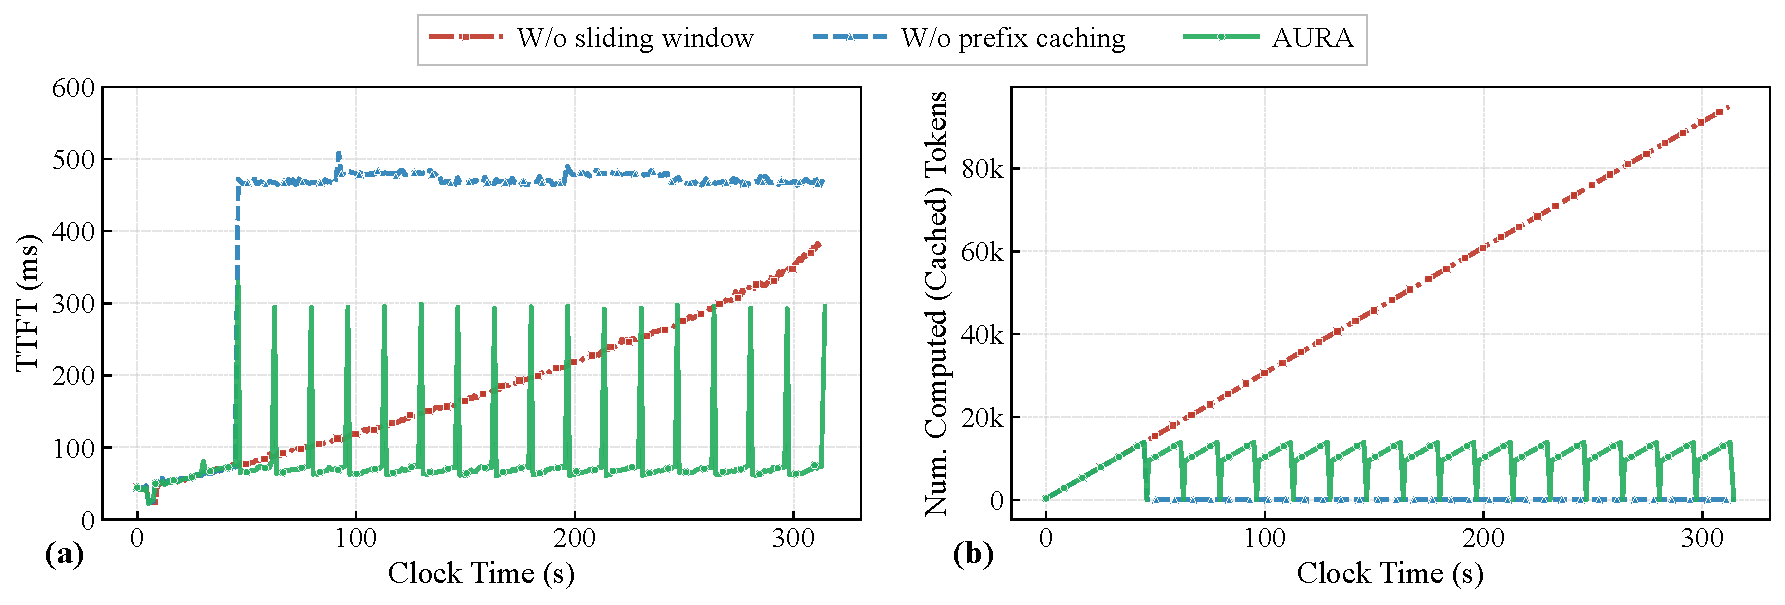
\includegraphics[width=\textwidth]{img/performance_qwen3vl_auro_paper.pdf}
    \caption{Inference performance of AURA. The figure compares (a) TTFT and (b) computed-token count across three settings: \textit{w/o sliding window}, \textit{w/o prefix caching}, and \textit{AURA}.}
    \label{fig:infer_pipeline}
\end{figure}


We implement the AURA inference engine on top of vLLM~\citep{vllm} and evaluate it in a latency-sensitive online video understanding setting. We use the same high-performance accelerators described in Section~\ref{subsec:training_detail} to deploy the system. We compare three configurations to isolate the contribution of our context management and cache reuse mechanisms: \textit{w/o sliding window}, which disables the sliding-window context management in Section~\ref{subsec:interactive_video_stream_context_management}; \textit{w/o prefix caching}, which disables prefix KV reuse by setting $N' = 1$; and \textit{AURA}, which enables the sliding window and uses $N' = 15$. For all settings, we use batch size 1, stream video continuously for 5 minutes at 2 FPS, and report time-to-first-token (TTFT), defined as the server-side latency between issuing a user query and receiving the first generated text token. A lower TTFT indicates better real-time responsiveness.


% Figure~\ref{fig:infer_pipeline} shows that \textit{AURA} achieves the lowest average TTFT, at 79\,ms, compared with 182\,ms for \textit{w/o sliding window} and 412\,ms for \textit{w/o prefix caching}. The left panel shows that disabling prefix caching keeps TTFT consistently high because the system repeatedly recomputes long prompt prefixes, whereas removing the sliding window causes latency to increase over time as the multimodal context accumulates. This trend is corroborated by the right panel, which reports the scheduler's computed-token count: without sliding-window pruning, the amount of active cached computation grows steadily throughout the stream, while \textit{AURA} keeps it bounded and therefore sustains substantially lower TTFT. Overall, these results show that real-time responsiveness in \textit{AURA} depends on both sliding-window context management and prefix cache reuse, with the former controlling context growth and the latter avoiding frequent redundant recomputation across successive streaming queries.

Figure~\ref{fig:infer_pipeline} shows that \textit{AURA} achieves the lowest average TTFT. The left panel shows that disabling prefix caching keeps TTFT consistently high because the system repeatedly recomputes long prompt prefixes, whereas removing the sliding window causes latency to increase over time as the multimodal context accumulates. This trend is corroborated by the right panel, which reports the scheduler's computed-token count: without sliding-window pruning, the amount of active cached computation grows steadily throughout the stream, while \textit{AURA} keeps it bounded and therefore sustains substantially lower TTFT. Overall, these results show that real-time responsiveness in \textit{AURA} depends on both sliding-window context management and prefix cache reuse, with the former controlling context growth and the latter avoiding frequent redundant recomputation across successive streaming queries.



\begin{table}[t]
  \renewcommand{\arraystretch}{1.2}
  \caption{End-to-end latency breakdown of AURA. ASR and TTS are averaged over 10 runs on a warmed-up engine. TTFT denotes the server-side time to the first output token of AURA, measured during a 5-minute continuous streaming session. We also report estimated first-sentence decode time. End-to-end latency is approximated as ASR + TTFT + first-sentence decode + TTS first-chunk latency.}
  \label{tab:inference_comparison}
  \centering
  \footnotesize
  \begin{tabular}{ccccc}
    \toprule
    ASR & TTFT & First-sent.\ decode & TTS first chunk & End-to-end \\
    \midrule
    84.2\,ms & 75.0\,ms & $\sim$60\,ms$^*$ & 93.0\,ms & $\sim$312.2\,ms \\
    \bottomrule
    \multicolumn{5}{l}{\scriptsize Decode speed: 7.3\,ms/tok ($\approx$137\,tok/s) \quad Avg.\ tokens/response: 12.6 \quad TTS RTF: 0.42} \\
    \multicolumn{5}{l}{\scriptsize TTFT: server-side mean over 5 mins (p50=74.6\,ms, p90=87.8\,ms, std=14.1\,ms)} \\
    \multicolumn{5}{l}{\scriptsize $^*$Estimated as $\sim$8\,tokens $\times$ 7.3\,ms/token for a typical first sentence.} \\
  \end{tabular}
\end{table}

\paragraph{End-to-end latency of AURA.}
We conduct independent latency analysis for each system component on the computing cluster described in Section~\ref{subsec:training_detail}. For inference deployment, we use two accelerators: one hosts both the ASR service (Qwen3-ASR-1.7B with vLLM as the inference backend) and the TTS service (Qwen3-TTS-12Hz-1.7B-Base with streaming synthesis), while the other hosts the main model (AURA with vLLM serving), with sliding-window attention and prefix caching enabled. For ASR, the test input consists of a 9.41-second Chinese speech command in MP3 format. For AURA, the test input consists of a 5-minute video at 2\,FPS. For TTS, the test input consists of a 40-character Chinese sentence. ASR and TTS are each evaluated independently over 10 runs on a fully warmed-up engine, whereas TTFT is measured during a 5-minute continuous streaming session to reflect steady-state performance under accumulated multi-turn context.

As shown in Table~\ref{tab:inference_comparison}, the ASR component transcribes the 9.41-second audio into text with an end-to-end latency of 84.2\,ms. For the main model, the server-side TTFT averages 75.0\,ms (p50\,=\,74.6\,ms, p90\,=\,87.8\,ms) over the 5-minute sustained streaming session, where sliding-window context management keeps the active context bounded and prefix caching avoids redundant recomputation across successive queries. During decoding, the generation speed is about 7.3\,ms per token (about 137\,tokens/s), and each response contains 12.6 generated tokens on average, corresponding to a total decoding time of about 100\,ms per response. However, because TTS operates in a sentence-level streaming fashion, audio synthesis can begin once the first sentence has been fully decoded. A typical first sentence is estimated to contain approximately 8 tokens, yielding an estimated first-sentence decode time of about 60\,ms; the remaining tokens are decoded in parallel with TTS synthesis and therefore do not contribute to the initial user-perceived latency. For streaming TTS, the first-chunk latency is highly stable at 93.0\,ms on average, with a real-time factor (RTF) of 0.42. Overall, the end-to-end latency from the user's speech input to the first spoken response is estimated to be approximately 312.2\,ms (ASR $\sim$84.2\,ms + TTFT $\sim$75\,ms + first-sentence decoding $\sim$60\,ms + TTS first chunk $\sim$93\,ms), which supports real-time conversational interaction.





\subsection{Research Question}

\paragraph{RQ1: Accuracy on Offline Video Benchmarks.}

To study how streaming-oriented training affects conventional offline video understanding, we compare AURA with its initialization model, Qwen3-VL-8B-Instruct, on three representative offline benchmarks, namely LongVideoBench~\citep{wu2024longvideobench}, MVBench~\citep{li2024mvbench}, and Video-MME~\citep{fu2025video}. We evaluate all three benchmarks with VLMEvalKit~\citep{duan2024vlmevalkit}, adhering to the original benchmark settings except that we use uniform 2 FPS sampling. This experiment is designed to answer a key question in our work: after optimizing the model for continuous streaming observation, selective silence, and delayed response in streaming scenarios, can it still preserve competitive offline understanding ability?

As shown in Table~\ref{tab:offline_rq1}, AURA achieves 58.8\% on LongVideoBench, 68.1\% on MVBench, and 65.1\% on Video-MME. Compared with its base model (Qwen3-VL-8B-Instruct~\citep{bai2025qwen3}), AURA remains particularly close on MVBench, while showing modest performance drops on LongVideoBench and Video-MME. Overall, these results indicate that streaming-oriented training enhances online interaction ability while largely preserving the model's offline video understanding capability.

\begin{table}[t]\Large
  \renewcommand{\arraystretch}{1.1}
  \caption{Offline benchmark comparison for studying the effect of streaming-oriented training on conventional offline video understanding. All results are reported in accuracy (\%).}
  \label{tab:offline_rq1}
  \footnotesize
  \centering
  \begin{tabular}{l|ccc}
    \toprule
    Method & LongVideoBench & MVBench & Video-MME \\
    \midrule
    Qwen3-VL-8B-Inst. & 61.9 & 69.0 & 68.6 \\
    AURA (Ours)  & 58.8 & 68.1 & 65.1 \\
    \bottomrule
  \end{tabular}
\end{table}

\begin{table*}[t]\Large
  \renewcommand{\arraystretch}{1.3}
  \caption{Ablation study on the training objective over OmniMMI in terms of accuracy (\%). We report averaged performance for Dynamic State Grounding (SG), Action Prediction (AP), Multi-turn Dependency Reasoning (MD), Speaker Identification (SI), Proactive Alerting (PA), and the overall average. The best and second-best results are highlighted in bold and underlined, respectively.}
  \label{tab:loss_rq2}
  \centering
  \setlength{\tabcolsep}{4pt}%
  \footnotesize
  \begin{tabular}{l|cccccc}
    \toprule
    Objective & \textbf{SG} & \textbf{AP} & \textbf{MD} & \textbf{SI} & \textbf{PA} & \textbf{All} \\
    \midrule
    Default Cross-Entropy Loss & \underline{22.7} & \underline{26.0} & \textbf{7.7} & \underline{25.5} & \underline{0.0} & \underline{16.4} \\
    Silent-Speech Balanced Loss (Ours) & \textbf{24.0} & \textbf{32.0} & \textbf{7.7} & \textbf{26.0} & \textbf{37.5} & \textbf{25.4} \\
    \bottomrule
  \end{tabular}
\end{table*}



    
    
    
    
    

\paragraph{RQ2: Effect of the Training Objective.}
To evaluate the training objective in Section~\ref{silent-speech_balanced_loss}, we conduct an ablation study on OmniMMI. Specifically, we train a variant of AURA with the same data, initialization, and training settings, but replace our objective with the default cross-entropy loss that uniformly optimizes all assistant messages. As shown in Table~\ref{tab:loss_rq2}, replacing our objective with the default loss substantially hurts overall performance: the overall average drops from 25.4\% to 16.4\%, and PA falls from 37.5\% to 0.0\%. Clear drops are also observed on State Grounding (SG), Action Prediction (AP), and Speaker Identification (SI).

Closer inspection shows that the model trained with the default loss tends to over-generate \texttt{<|silent|>}, remaining silent at every time step in PA. For non-proactive interaction metrics, the degradation is also consistent with our supervision-selection design: under sliding-window truncation, earlier non-silent assistant responses may no longer be fully supported by the preserved visual and history context, so uniformly supervising all assistant messages can introduce insufficiently grounded targets and increase hallucination risk. 
These results directly reflect the problems that our objective is designed to address: it reweights silent messages to prevent excessive silence and supervises only the final non-silent assistant message to reduce hallucinations.

